\documentclass[12pt, letterpaper]{article}
\usepackage[utf8]{inputenc}
\usepackage{graphicx} % inserer des figures
\usepackage{hyperref} % lien html
\usepackage{fancyvrb} % Vertbatim avec une majuscule
\usepackage{array} % tableaux
\usepackage{float}
\usepackage{subcaption}

\title{Traitement du signal et des images : Projet mini boîte a outils pour traitement d'image}
\author{Chaolei Cai
\\
    \multicolumn{1}{
        p{.7\textwidth}}{\centering\emph{Université Paris Vincennes St-Denis\\
  UFR mathématiques, informatique, technologies sciences de l'information\\}
  L3 Informatique}
}
\date{\today}
\begin{document}

 
\begin{titlepage}
    \maketitle
\end{titlepage}

\tableofcontents

\section{Présentation}
Ce document est mon rapport pour le cours de Traitement du signal et des images enseigné par M.Boubchir au 3ème année de 
la Licence Informatique.\\
Le but du projet est donc crée un petit programme avec une interface \\graphique, permettant ainsi de 
visualiser rapidement certain traitement applicable sur l'image.\\


\section{Dépendances}
Le projet a été écrite en Scilab 6.0.2, il nécessite la librairie IPCV (Image Processing and Computer Vision Toolbox).\\
L'interface graphique a été écrite via l'outils guibuilder, si vous rencontrez des problèmes d'exécution, vérifier la version de Scilab 
que vous possèdez et vérifier la présence de ces 2 librairies. Recemment, il y a eu une mise à jour de Scilab en 6.1.0, je n'ai 
pas encore tester le programme sous cette version car le developpement a été faite en 6.0.2\\
La compatibilité avec une version Scilab 5.X.X est sans doute possible, mais il faudra charger le module 
SIVP (Scilab Image and Processing Video).\\
Il faut patienter un brief moment après le click sur un boutton car les calcules sont longues.


\section{Apperçue génerale de l'interface}

\begin{figure}[h!]
    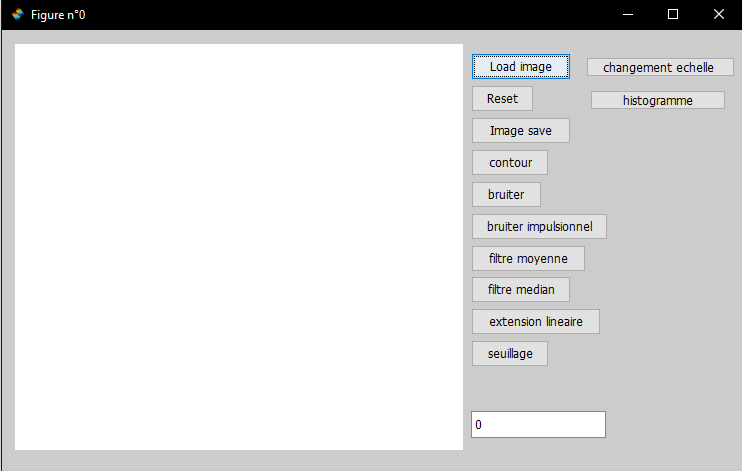
\includegraphics[width=\linewidth]{img/fig1.png}
    \caption{Page d'accueil}
    \label{fig:accueil}
\end{figure}

Voici donc la page d'accueil de mon programme, pour ouvrir cette interface, ouvrez Scilab, depuis le navigateur de fichier, 
il faut aller vers le repertoire où se trouve "gui.sce" et "traitement.sce".\\
Depuis la console de scilab, tapez la commande suivante "exec gui.sce".

\section{Présentations des fonctionalités}
\subsection{Load image, Reset, Image save}
Comme leurs noms l'indiquent, ces 3 bouttons permettent de charger une image, recharger l'image et de sauvergarder l'image.
Dès lors, une interface de navigateur de fichier s'affiche, cette fonctionalités ont été réalisé via les fonctions "uigetfiles" et "uiputfiles"
\begin{figure}[h!]
    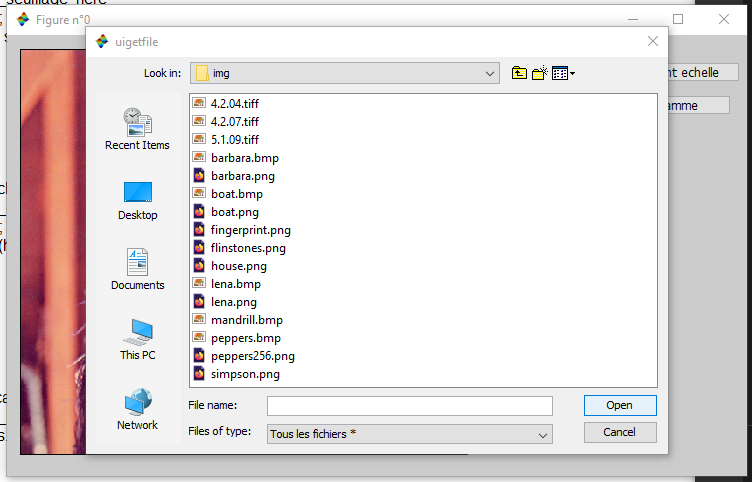
\includegraphics[width=\linewidth]{img/fig2.png}
    \caption{Interface de chargement \& sauvergarde }
    \label{fig:loading}
\end{figure}
 

\subsection{Contour}
Le boutton contour permet de d'afficher le contour des formes contenue dans l'image, via la norme du gradient discret, 
c'est une manière possible d'implémenter le filtre de Sobel enseigné en cours.

\subsubsection{Norme du gradient}
La fonction suivante renvoie la norme du gradient discret en fonction d'une image, il faut alors préciser sa position i, j. 
Les dimensions sizeX, sizeY et sizeZ de l'image, ainsi qu'une constance à appliquer pour pondérer le résultat.

\begin{Verbatim}[numbers=left,xleftmargin = 5mm]
    function [v] = norme_gradient(img,i,j, sizeX, sizeY, sizeZ,cst)
    if i < sizeX then
        a = img(i+1, j, sizeZ);
    else
        a = 0;
    end
    
    if i > 1 then
        b = img(i-1, j, sizeZ);
    else
        b = 0;
    end

    if j < sizeY then
        c = img(i, j+1, sizeZ);
    else
        c = 0;
    end

    if j > 1 then
        d = img(i, j-1, sizeZ);
    else
        d = 0;
    end
    v = cst * sqrt( (a-b)**2 + (c-d)**2);
endfunction
\end{Verbatim}

\begin{Verbatim}[numbers=left,xleftmargin = 5mm]
function [M] = im_contour(img, cst)
[sizeX, sizeY, sizeZ] = size(img);
M = zeros(sizeY, sizeX,sizeZ);
for k = 1 :sizeZ
    for i = 1 :sizeY
        for j = 1:sizeX
            //disp(i,j);
            M(i,j, k) = norme_gradient(img, i, j, sizeX, sizeY, k, cst);
        end
    end
end
endfunction
\end{Verbatim}
Enfin la fonction im\_contour renvoie l'image du contour à partir d'une image et du coefficient à appliquer.

\begin{figure}[h!]
    \centering
    \begin{subfigure}[b]{0.7\linewidth}
      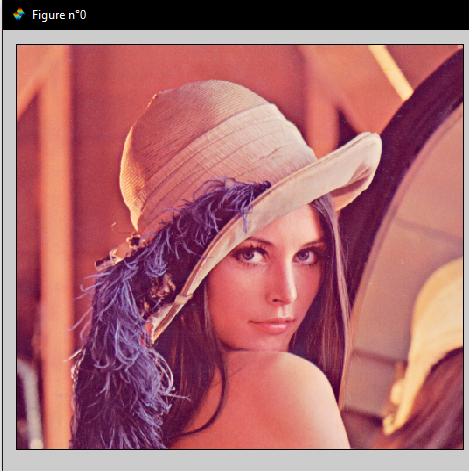
\includegraphics[width=\linewidth]{img/fig3.PNG}
      \caption{Image initial: 4.2.04.tiff}
    \end{subfigure}
    \begin{subfigure}[b]{0.7\linewidth}
      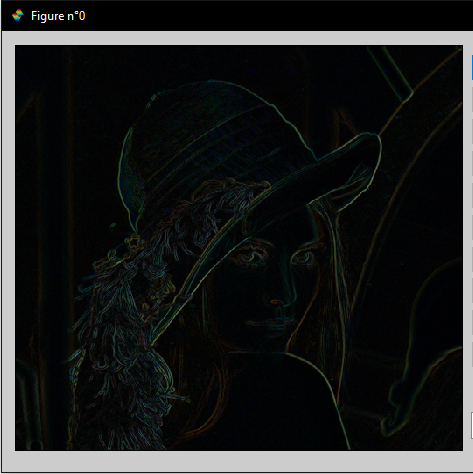
\includegraphics[width=\linewidth]{img/fig4.PNG}
      \caption{L'image du contour après traitement}
    \end{subfigure}
    \caption{Contour sur une image couleur}
    \label{fig:contour1}
\end{figure}
\begin{figure}[h!]
    \centering
    \begin{subfigure}[b]{0.7\linewidth}
      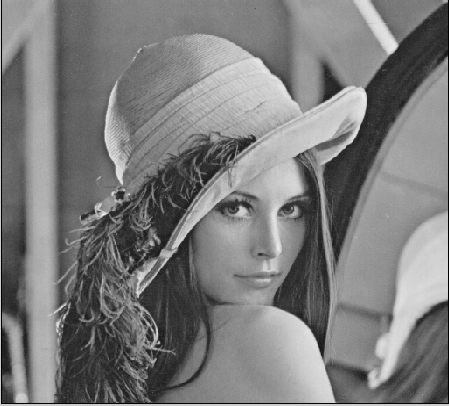
\includegraphics[width=\linewidth]{img/fig5.PNG}
      \caption{Image initial: lena.png}
    \end{subfigure}
    \begin{subfigure}[b]{0.7\linewidth}
      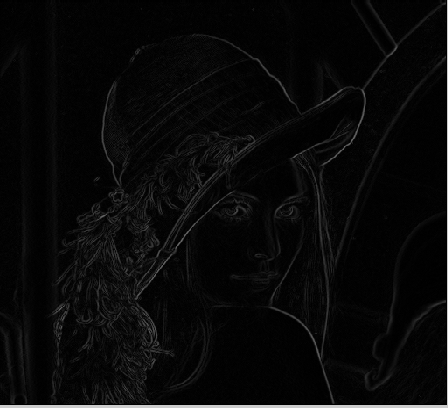
\includegraphics[width=\linewidth]{img/fig6.PNG}
      \caption{L'image du contour après traitement}
    \end{subfigure}
    \caption{Contour sur une image noire et blanc}
    \label{fig:contour1}
\end{figure}
La fonction ne fait pas de distinction quelque soit la nature de l'image, il peut être en noire et blanc ou en couleur,
 cenpendant, le traitement des images en couleur est plus lente car nécessite plus de calcules.


\subsection{Bruitage}
Pour le bruitage, 2 options sont disponible, la première est le bruitage constant, il faut saisir une valeur dans le champs de saisit en bas, 
puis cliquer sur le boutton "bruiter", la fonction ajoute un bruit géneré aléatoirement et pondérer par la valeur saisit.\\
Le bruit impulsionnel est plus sophistiqué, ce n'est plus une valeur comme paramètre de bruit mais un pourcentage, la fonction 
applique un bruit aléatoire sur cette pourcentage d'image aléatoirement, par exemple si la valeur saisit est de 50, 
alors 50 pourcentage de l'image recevront un bruit aléatoire.
\begin{Verbatim}[numbers=left,xleftmargin = 5mm]
    function [Ub] = bruite(U, s)
    // Description of bruite(U, s)
        Ub = rand(size(U,1), size(U,2),size(U,3), 'normal');
        Ub = Ub * s + U;
    endfunction
    
    
    function [Uimp] = bruite_imp(U, p)
    // Description of bruite(U, s)
    I = rand(U);
    //disp(I);
    Uimp = 255*rand(U).*(I <p/100) + (I>=p/100).*U;
    endfunction    
\end{Verbatim}


\begin{figure}[h!]
    \centering
    \begin{subfigure}[b]{0.7\linewidth}
      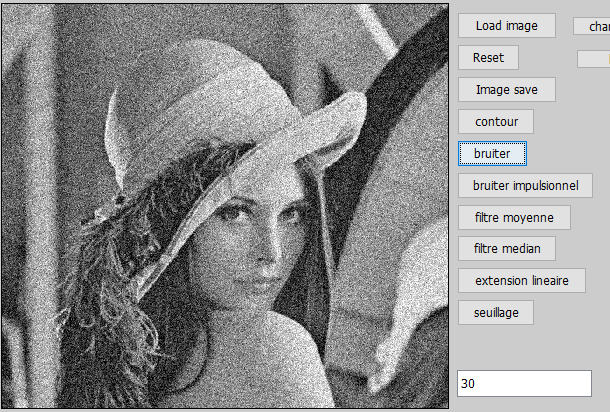
\includegraphics[width=\linewidth]{img/fig7.PNG}
      \caption{Bruitage basique}
    \end{subfigure}
    \begin{subfigure}[b]{0.7\linewidth}
      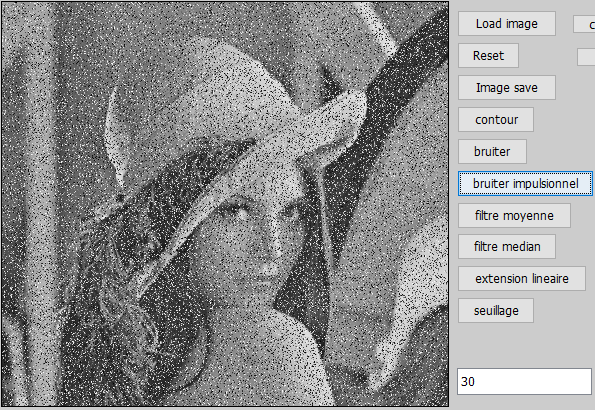
\includegraphics[width=\linewidth]{img/fig8.PNG}
      \caption{Bruitage impulsionnel}
    \end{subfigure}
    \caption{Bruitages}
    \label{fig:bruitages}
\end{figure}

\subsection{Débruitage via la méthode de filtre}
Le débruitage est possible via 2 filtre: le filtre moyenne ou le filtre médian, il faut faire attention au champs de saisit,
car le débruitage nécessite la dimensions du filtre, par exemple la valeur 2 donneras un filtre de 2 * f +1 soit 5x5 en dimensions.
Plus le filtre est grand, plus la fonction est longue en pour ses calculs.
\begin{Verbatim}[numbers=left,xleftmargin = 5mm]
function [M] = im_moyenne(U,f)
// Description of im_moyenne(U, f)
nb = (2*f +1)^2;
[sizeY, sizeX, sizeZ] = size(U);
M = zeros(U);
for k = 1:sizeZ
for i = 1:sizeY
    for j = 1:sizeX
        M(i,j, k) = sum(im_extract(U, i, j , f, k))/nb;
    end
end
end
endfunction

function [M] = im_median(U,f)
    // Description of im_median(U, f)
    nb = (2*f +1)^2;
    [sizeY, sizeX, sizeZ] = size(U);
    M = zeros(U);

    for k = 1:sizeZ
    for i = 1:sizeY
        for j = 1:sizeX
            M(i,j,k) = median(im_extract(U, i, j , f, k));
        end
    end
end
endfunction
\end{Verbatim}
sum et médian sont des fonctions de base de Scilab, im\_extract est une fonction que j'ai écrite pour extraire une sous matrice depuis ses cordonnées et ses dimensions.
\begin{figure}[h!]
    \centering
    \begin{subfigure}[b]{0.7\linewidth}
      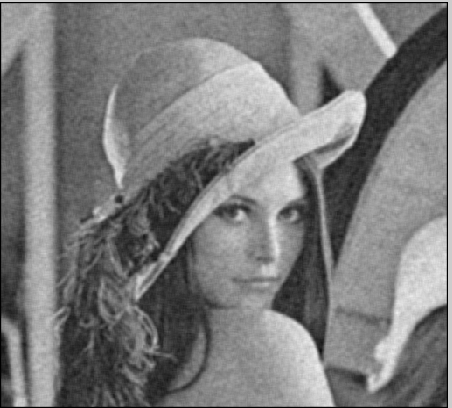
\includegraphics[width=\linewidth]{img/fig9.PNG}
      \caption{Filtrage moyenne sur un filtre de 5x5}
    \end{subfigure}
    \begin{subfigure}[b]{0.7\linewidth}
      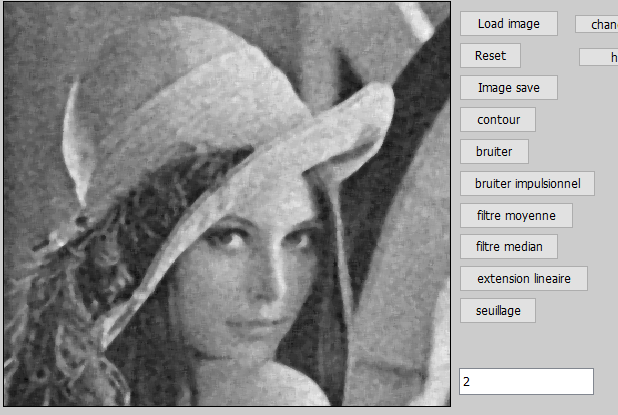
\includegraphics[width=\linewidth]{img/fig10.PNG}
      \caption{Filtrage median sur un filtre de 5x5}
    \end{subfigure}
    \caption{Application des 2 filtres sur une image bruité}
    \label{fig:contour1}
\end{figure}

\subsection{Extension linéaire}
Extension linéaire est une technique qui permet d'améliorer le contraste d'une image, il permet notamment d'étirer 
l'histogramme d'une image sur ses valeurs limites non utilisé.

\begin{figure}[h!]
    \centering
    \begin{subfigure}[b]{0.7\linewidth}
      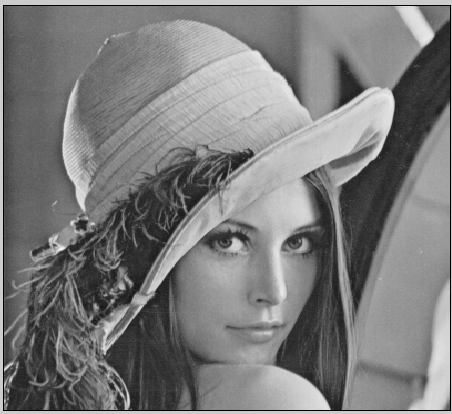
\includegraphics[width=\linewidth]{img/fig11.PNG}
      \caption{Image initial}
    \end{subfigure}
    \begin{subfigure}[b]{0.7\linewidth}
      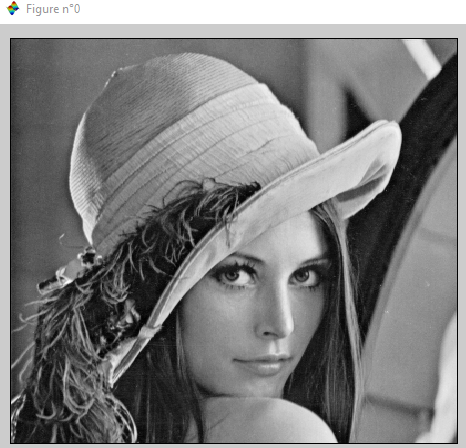
\includegraphics[width=\linewidth]{img/fig12.PNG}
      \caption{Image après filtrage}
    \end{subfigure}
    \caption{Extension linéaire sur une image noire et blanc}
    \label{fig:extend1}
\end{figure}
\begin{figure}[h!]
    \centering
    \begin{subfigure}[b]{0.7\linewidth}
      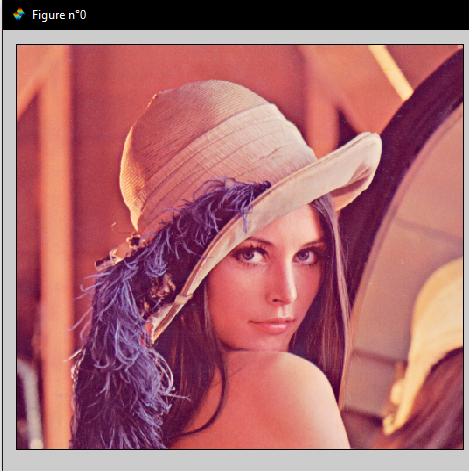
\includegraphics[width=\linewidth]{img/fig3.PNG}
      \caption{Image initial}
    \end{subfigure}
    \begin{subfigure}[b]{0.7\linewidth}
      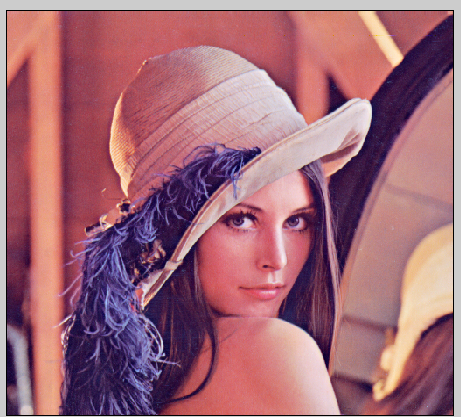
\includegraphics[width=\linewidth]{img/fig13.PNG}
      \caption{Image après filtrage}
    \end{subfigure}
    \caption{Extension linéaire sur une image couleur}
    \label{fig:extend2}
\end{figure}

\begin{Verbatim}[numbers=left,xleftmargin = 5mm]
function [I] = extension_lineaire(U)
// Description of extension_lineaire(U)
LUT = zeros(256, size(U,3));
for k = 1 : size(U,3)
for ng = 1:256
    LUT(ng, k) = 255 * (ng - min(U(:,:,k))) / (max(U(:,:,k)) - min(U(:,:,k)));
    //mprintf("ng = %d , lut(ng) = %d\n", ng, 255 * (ng - min(U(:,:,k))) / (max(U(:,:,k)) - min(U(:,:,k))));
end
end
I = zeros(U);
for k = 1: size(U,3);
for i = 1: size(U,1)
    for j = 1:size(U,2)
        I(i,j,k) = LUT(U(i,j,k), k);
    end
end
end

endfunction
\end{Verbatim}
L'extension linéaire se fait par une look up table, on créer d'abord cette LUT via les valeurs minimal et maximal,
puis une image resultant est géneré via la consultation de cette LUT.

\subsection{Seuillage}
Le Seuillage est une technique qui étire l'image vers les valeurs limites selon une valeur de réference, on obtiens alors une image noire et blanc,
cette fonctionalités ne marche que pour pour les images en niveau de gris.

\begin{figure}[h!]
    \centering
    \begin{subfigure}[b]{0.7\linewidth}
      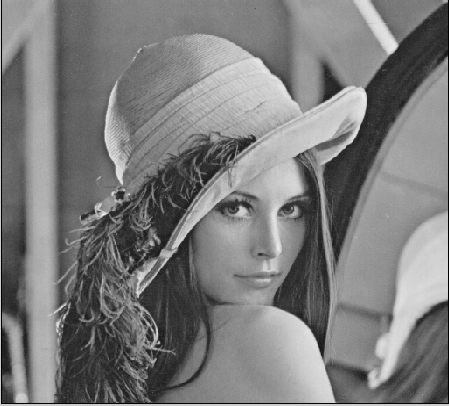
\includegraphics[width=\linewidth]{img/fig5.PNG}
      \caption{Image initial}
    \end{subfigure}
    \begin{subfigure}[b]{0.7\linewidth}
      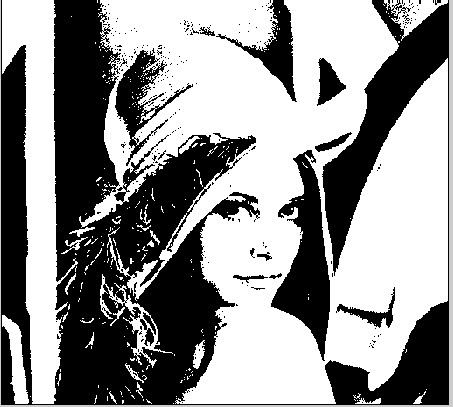
\includegraphics[width=\linewidth]{img/fig14.PNG}
      \caption{Image après seuillage}
    \end{subfigure}
    \caption{Résultat du seuillage}
    \label{fig:seuil}
\end{figure}

\subsection{changement d'echelle}
Cette fonctionalités permet de change l'échelle de l'image, cenpendant il ne donne pas de résultat sur l'interface graphique,
essayer de sauvergarder l'image et de comparer ainsi les résultats.

\subsection{histogramme}
Cette fonctionalités permet d'afficher l'histogramme d'une image quelque soit sa nature.
\begin{figure}[h!]
    \centering
    \begin{subfigure}[b]{1\linewidth}
      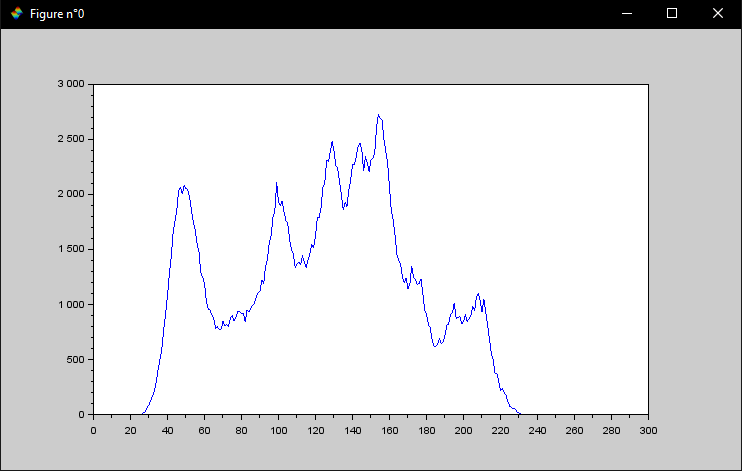
\includegraphics[width=\linewidth]{img/fig15.PNG}
      \caption{histogramme noire et blanc}
    \end{subfigure}
    \begin{subfigure}[b]{1\linewidth} 
      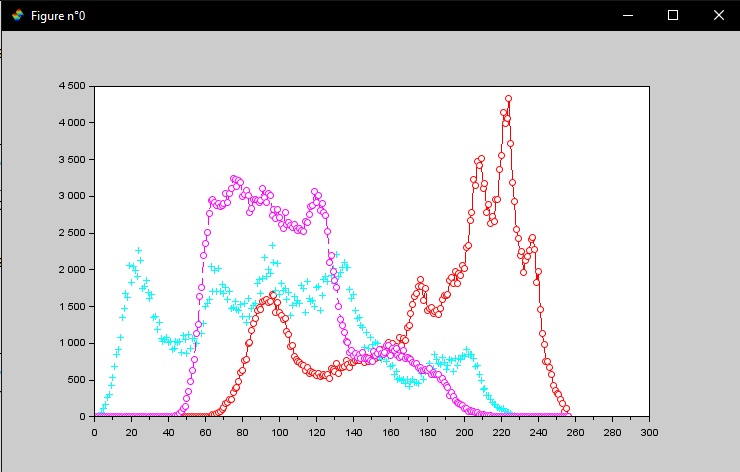
\includegraphics[width=\linewidth]{img/fig16.PNG}
      \caption{histogramme couleur}
    \end{subfigure}
    \caption{Résultat de histogramme}
    \label{fig:histo}
\end{figure}

\end{document} 